\documentclass{article}
\usepackage{parskip}
\usepackage{pdfpages}
\usepackage{hyperref}
\usepackage{amsmath}
\usepackage[margin=.6in]{geometry}

\begin{document}
\includepdf[pages=2-3]{slides}
Usually we would say that when the car is close to another car we start breaking. We want to pass our ability to determine "too close" to the car so that it can detect it. We can't just have a binary value of break, no break since everything is continuous.

\includepdf[pages=4]{slides}
In real life we drive by evaluating on a spectrum rather than binary values.

\includepdf[pages=5]{slides}
English is not very good at crisp descriptors.

\includepdf[pages=6-11]{slides}

\includepdf[pages=12]{slides}
We have the set of all things we are considering for the given context, called the \textbf{universe of discourse}. Within that set we get a fuzzy set. That fuzzy set has an inner part that is known to belong to the set and an outer boundry that is fuzzy.

\includepdf[pages=13-14]{slides}
We define a \textbf{membership function} that helps us determine if an item belongs in the set as a degree. Its important to note that the membership function does not output probability but the grade of possibility.

\includepdf[pages=15-17]{slides}
We can represent the membership function as a discrete function or as an continuous function. This will be determined by the universe in which we are working

\includepdf[pages=18-23]{slides}
Membership functions are bitchin.

Triangular and trapezoidal membership functions are the cheapest to calculate, but they are non-differentiable which turns out to be very important later on.

\includepdf[pages=24-26]{slides}
Union and intersection of fuzzy sets work a bit weirdly. For now we are just going to use these equations but a better definiton will be provided.

\includepdf[pages=27]{slides}
Lets consider this discrete fuzzy set A. To find the compliment we go through each value in the universe of discourse and subtract each value in the set A from 1 (if there is no value in the set A for the entry its "value" is 0).

\textbf{Important note:} A/B notation is not division, but equivalent to (B,A) coordinates. Basically given input B we get output A from the given function. The pluses denote set addition not mathematical addition.

\includepdf[pages=28-30]{slides}

\includepdf[pages=31-34]{slides}

\includepdf[pages=35]{slides}
Here we have three axioms that we must satisfy inorder to have a fuzzy compliment. There are infintely many operatators that could provide a compliment.

\textbf{KNOW THIS!!!!!}


\includepdf[pages=36-37]{slides}
Here is the criteria required for a intersection operator.

\textbf{KNOW THIS!!!!}

\includepdf[pages=38]{slides}
I don't really understand the first part of this slide.

Here are four basic forms of intersection functions. We want to think of the intersection as a sort of minimum. There are infinite number of T-norm operators here are just basic ones.

\includepdf[pages=39]{slides}
\includepdf[pages=40]{slides}
We call the union operator the S-norm or the T-conorm operator.

S-norm and T-norm must follow DeMorgan's law.

The compliment of (a times S-norm times b) is equal to the compliment of a times T-norm times the compliment of b

\includepdf[pages=41]{slides}
We defined the T norm as the minumum function so when we sub it into DeMorgan's equation we can prove that the S-norm is the max function.


\includepdf[pages=42]{slides}
More properties

\textbf{KNOW THIS!!!}

\includepdf[pages=43]{slides}
The algrebraic sum is $a+b-ab$ because we always want the sum to be in [0,1). WATCH THIS, its a common mistake and with fuck up everything.

\includepdf[pages=44]{slides}
\includepdf[pages=45]{slides}
A set A is fully included in a set B if the the membership function of A is strictly less than the membership function of B. We can limit this over a set interval.

\includepdf[pages=46]{slides}
With fuzzy sets we can have fuzzy inclusion. Basically the grade of inclusion is given to sets.

\includepdf[pages=47-49]{slides}

\includepdf[pages=50]{slides}
Dilation and contraction are other operations applied to the fuzzy set.

Dilation is denoted as $A^{\frac{1}{2}}$  gives a more elongated membership function over the universe. The integral in the equation is only used in the continuous case, it might not always apply. This gives us richness of the values. We use it to say its more or less "adjective". It increases the membership grade of elements that have small grades.

Contraction is basically the opposite of dilation.

Helpful slides: \href{http://web.cecs.pdx.edu/~mperkows/CLASS_479/LECTURES479/FL001.PDF}{Helpful slides}

\includepdf[pages=51-55]{slides}

In an assignment if not specified:
\begin{itemize}
	\item T-norm = min
	\item S-norm = max
	\item Compliment = 1-value
\end{itemize}

\includepdf[pages=56]{slides}
There are many different types of implication operators. They are very similar to the intersection operator in terms of input and output but they mean very different things.

He kind of defined it as a transition between fuzzy sets. It was a bit unclear.


helpful slides: \href{http://www.intelligent-systems.info/classes/ee509/8.pdf}{Helpful slides}

\includepdf[pages=57]{slides}
This is an example of the larsen implication operator where both fuzzy sets have a triangle membership function.

\includepdf[pages=58]{slides}
\includepdf[pages=59]{slides}
\includepdf[pages=60]{slides}
The height of a fuzzy set is the highests value of its membership function. The modal point is the value at which the max occurs.

\includepdf[pages=61]{slides}
\includepdf[pages=62]{slides}
The crisp set (aka support set) is the set of all points where the membership function has a nonzero value.

\includepdf[pages=63]{slides}
This is the generalized bell membership function. This is considered the richest membership function. You can see from this graph that it has a crisp set, but also that its modal point is actually a set of points since the graph has a plateau of highest points.

The \textbf{core} is the set of points at which the function has its highest values (aka the set of modal points). The \textbf{cross over points} are the points where the membership function has the value of 0.5. The \textbf{alpha cut} is the crisp set at which the membership function has values higher than some given $\alpha$.

\includepdf[pages=64]{slides}
The closeness to grade 0.5 - the fuzziest part of the membership function is at the cross over point. If we go lower than 0.5 we have values that are "low" so we are almost exiting the fuzzy set and if we go up then we are reaching values that are close to being in the fuzzy set, but at 0.5 we aren't sure what to do.

Distance from 1/2 cut - this is a specific alpha cut at 0.5 which is very similar to the above one.

\includepdf[pages=65-67]{slides}
The measure of fuzziness is that total amount of fuzziness in your system. It is represented as an integral of a fuzziness measurement function.

The closeness to 0.5 is super simple, we just integrate across a function for the difference.

The closeness to 1/2 cut its found by integrating across the absoute value of the difference between the membership value and its corresponding alpha cut at 0.5

The inverse distance of the compliment works out to be just literally the integral of the absolute value of the difference between the membership value and its compliment.

We have a relationship between these

\includepdf[pages=68-79]{slides}
important note: remember that we are using different functions. there is no division or addition going on here,

Here we have a discrete fuzzy set A. We apply to it some mapping $f()$. The output of this mapping is a discrete fuzzy set B. You can see that the y values of the pairs is not changing, just the x values, thus the height is the same.

Where we have multiple x's for the same y we take the maximum of them.

\includepdf[pages=80]{slides}
\includepdf[pages=81]{slides}
Here part of the mapping is bijective and part is not. Weird.

\includepdf[pages=82-86]{slides}
Given a relation R. We use a projection to eliminate the set Y by projecting it onto X. We go across the whole spectrum of y and project its max value onto x.  The next two slides show such projections.

Usually the total projection is a constant.

We can expand this out to the nth dimension. In this case the first projection would be

\begin{equation}
	\mu_{R}(x_1 ... x_n) = \vee_{x_n} \max[\mu_{R}(x_1 ... x_{n-1}))]
\end{equation}

We keep going for the second, third, and so on until you get the total projection.


\includepdf[pages=87-89]{slides}
Say we take the value 0.2 at y=6 x=3, this value is like a a three dimensional modal representing a system with two control variable. When we set them to 6 and 3 we got the value 0.2. So the matrix in this example R represents a three dimensional graph.

So we take the maximum y value for instances where x = 1. Basically going across the top row, so in this case 1.0. Repeat for each row. This is where $R^1$ comes from.

The second projection works the same way but sideways. We just take the max of each column.

These values get projected onto the 3d graph by having $R^1$ on the x axis and $R^2$ on the y axis.

The total projection we take the max of the values in $R^1$ or $R^2$ which in this case is 1.0. This is a single point, one dimensional (well technically 0 dimensional but its easier to think of it as one).

So a projection is a reduction of order in the fuzzy dimensions.

\includepdf[pages=90]{slides}
The cylindrical expansion is the opposite of projections, it increases order.

We take the elements from the initial projections. In this example $R^1$ and $R^2$ are the same as in the previous example. These are expanded out to match the initial dimensions of the relation by replicating across columns/rows.

The cylindrical expansion does not undo a projection. Once you projection you cannot get back to the initial relation.

\includepdf[pages=91]{slides}
\includepdf[pages=92]{slides}
The knowledge base is just the mathematical representation of a system composed of rules. We create a function or descriptive value for each rule our system gives us. Say we have 3 potential temperatures, 3 pressure, and 3 humidities we will have $3 \times 3 \times 3 = 27$ rules for our system. Each of these rules are fuzzy relations. If the temperature is high then the air conditioner is on, and so on. This is an implication operator (T-norm). We want a model that encapsulates all potential input types because we don't know what we will get.

\includepdf[pages=93]{slides}
\includepdf[pages=94]{slides}
The context is the current set of input data. The system processes the context and decides what action it needs to do. It keeps repeating this cycle.
\begin{itemize}
	\item Context = D (for data)
	\item Rules = K (for knowledge)
	\item Relation = I (for inference)
\end{itemize}

The membership is of the inference is
\begin{equation}
	\mu_I = \sup_y\{\min[\mu_D, \mu_K]\}
\end{equation}

The super min (or max) is the min value tending to the absolute min.

\emph{Look up what the sup min composition operator is}

Another way to compose thins is the sup produce.

\emph{look this up too}

\includepdf[pages=95-96]{slides}
A process takes input C and outputs A. The output A feeds into a controller that has to make decisions, it takes input A and outputs C. We then define a relation $R=A\implies C$.

We take some measurements and get a context of $A_0$. The controller maps this to R using a composition rule, doing so it decides what to do.

\includepdf[pages=97-99]{slides}
Now we are trying to compose relations, a relation of relations if you will.

\includepdf[pages=100-106]{slides}
Remember the projection onto x is the max of all y values for a given x in the relation (max of rows).

\includepdf[pages=107-124]{slides}

























\end{document}
